
% =========================================================================================
% HOMEWORK TEMPLATE %===================================================================
% =========================================================================================

% =========================================================================================
% LaTeX SETUP %============================================================================
% =========================================================================================
 \documentclass[tikz]{standalone}

  \usetikzlibrary{automata,positioning}					% Change "article" to "report" to get rid of page number on title page
\usepackage{amsmath,amsfonts,amsthm,amssymb,empheq}
\usepackage{setspace}
\usepackage{Tabbing}
\usepackage{fancyhdr}
\usepackage{lastpage}
\usepackage{extramarks}
\usepackage{chngpage}
\usepackage{soul,color}
\usepackage{graphicx,float,wrapfig}
\usepackage[retainorgcmds]{IEEEtrantools}

% =========================================================================================
% TikZ SETUP %==============================================================================
% =========================================================================================
\usepackage{tikz}
\usepackage{verbatim}
\usetikzlibrary{shapes,arrows,positioning,calc,scopes,angles,quotes}
\usetikzlibrary{decorations.markings}

% =========================================================================================
% MARGINS %===============================================================================
% =========================================================================================
%\topmargin=-1in      
%\evensidemargin=0in     
%\oddsidemargin=0in      
%\textwidth=6.5in        
%\textheight=9.0in       
%\headsep=0.25in         

% =========================================================================================
% ASSIGNMENT INFORMATION %===============================================================
% =========================================================================================
\newcommand{\hmwkTitle}{Homework\ \#5}
\newcommand{\hmwkDueDate}{ March\ 9,\ 2016}
\newcommand{\hmwkClass}{EE\ 324}
\newcommand{\hmwkClassTime}{Munk}
\newcommand{\hmwkClassInstructor}{Prof. Jens}
\newcommand{\hmwkAuthorName}{Blair Munro}

% =========================================================================================
% HEADER & FOOTER %=======================================================================
% =========================================================================================

% =========================================================================================
% BEGIN DOCUMENT %=======================================================================
% =========================================================================================

\begin{document}


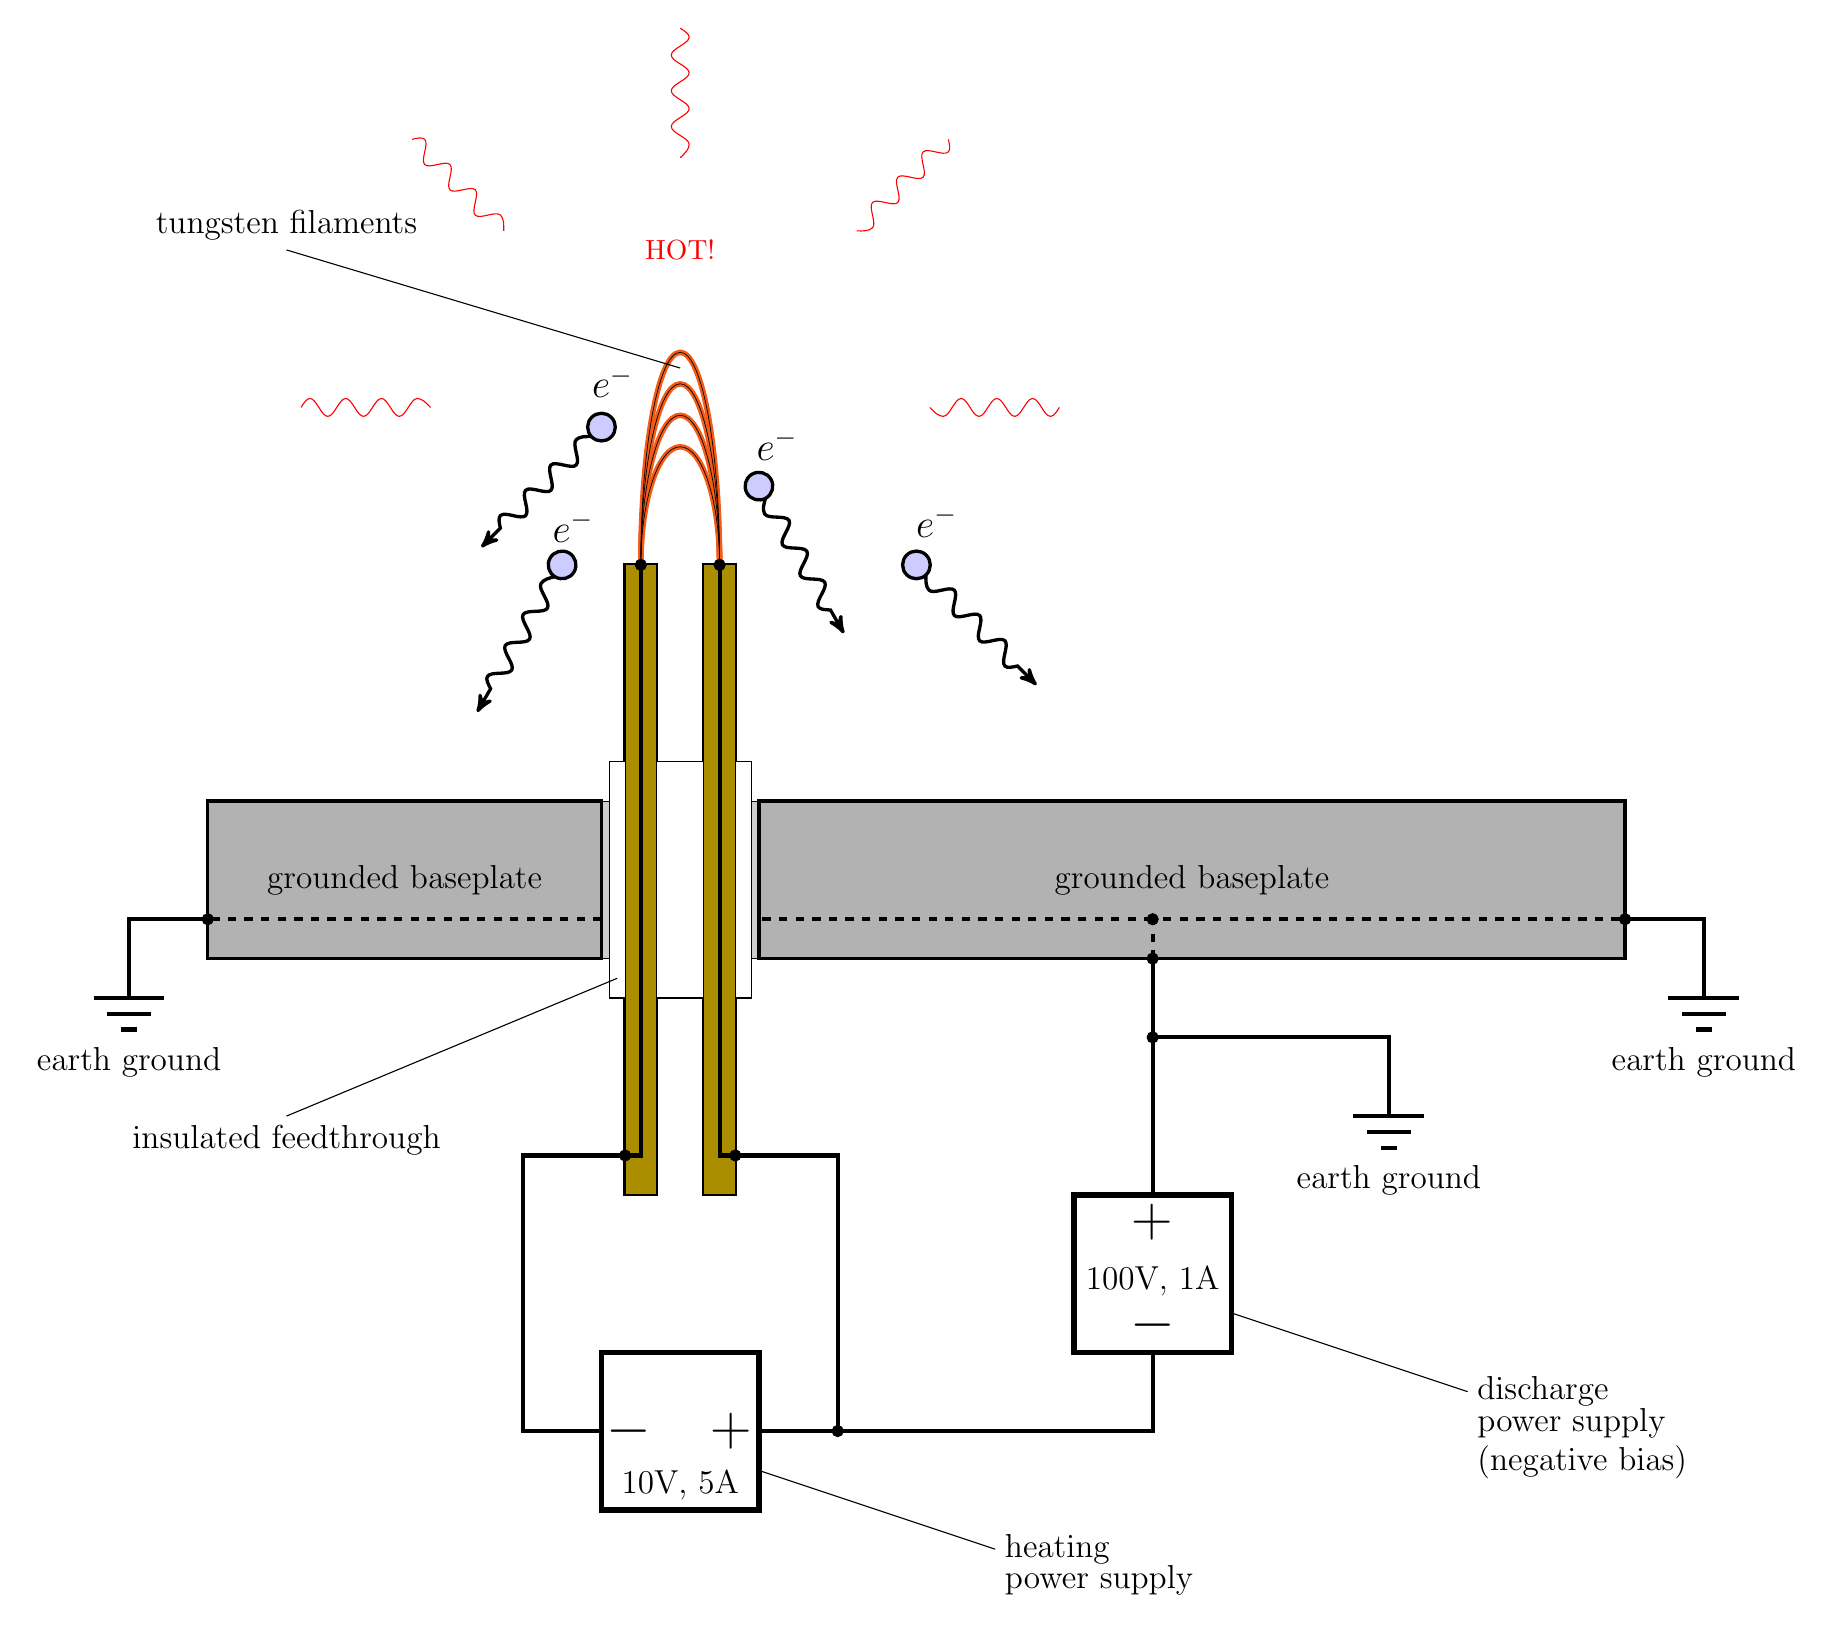
\begin{tikzpicture}[
	scale=1,
	vector/.style={very thick,->, >=latex},
	axis/.style={very thick, ->, >=stealth'}]
	
	\filldraw[fill=gray!60] (0,0) rectangle (5,2);
	\filldraw[fill=gray!60] (7,0) rectangle (18,2);
	\filldraw[fill=gray!40] (5,0) rectangle (7,2);
	\draw [very thick] (0,0) rectangle (5,2);
	\draw [very thick] (7,0) rectangle (18,2);
	\draw [very thick] (5.3,-3) rectangle (5.7,5);
	\draw [very thick] (6.7,-3) rectangle (6.3,5);
	\draw (6,9) node [color=red] {HOT!};

	\draw[fill=white](5.1,-0.5)rectangle(6.9,2.5);

	\draw [line width=2pt, color=yellow!30!red]  (5.5,5) arc (180:0:.5 and 1.5);
	\draw [line width=2pt, color=yellow!30!red]  (5.5,5) arc (180:0:.5 and 1.9);
	\draw [line width=2pt, color=yellow!30!red]  (5.5,5) arc (180:0:.5 and 2.3);
	\draw [line width=2pt, color=yellow!30!red]  (5.5,5) arc (180:0:.5 and 2.7);
	\filldraw[fill={rgb:red,2;green,1.5;yellow,1}] (6.7,-3) rectangle (6.3,5);
	\filldraw[fill={rgb:red,2;green,1.5;yellow,1}] (5.3,-3) rectangle (5.7,5);
	\draw [line width=0.25pt]  (5.5,5) arc (180:0:.5 and 1.5);
	\draw [line width=0.25pt]  (5.5,5) arc (180:0:.5 and 1.9);
	\draw [line width=0.25pt]  (5.5,5) arc (180:0:.5 and 2.3);
	\draw [line width=0.25pt]  (5.5,5) arc (180:0:.5 and 2.7);
	
	\begin{scope}[shift={(9,5)},rotate=-45]
	\draw[axis,x=0.75ex,y=0.75ex] (1.5,0) sin (3,-1) cos (4,0)sin (5,1) cos (6,0) sin (7,-1) cos (8,0)sin (9,1) cos (10,0) sin (11,-1) cos (12,0)sin (13,1) cos (14,0) sin (15,-1) cos (16,0)--(19,0);
	\draw[very thick,fill=blue!20!white,] (0,0)circle(5pt) (-.25,.05)node[above right]{\Large{$e^-$}}; 
	\end{scope}
	\begin{scope}[shift={(7,6)},rotate=-60]
	\draw[axis,x=0.75ex,y=0.75ex] (1.5,0) sin (3,-1) cos (4,0)sin (5,1) cos (6,0) sin (7,-1) cos (8,0)sin (9,1) cos (10,0) sin (11,-1) cos (12,0)sin (13,1) cos (14,0) sin (15,-1) cos (16,0)--(19,0);
	\draw[very thick,fill=blue!20!white,] (0,0)circle(5pt) (-.25,-.05)node[above right]{\Large{$e^-$}}; 
	\end{scope}
	\begin{scope}[shift={(7,6)},shift={(-2.5,-1)},rotate=-120]
	\draw[axis,x=0.75ex,y=0.75ex] (1.5,0) sin (3,-1) cos (4,0)sin (5,1) cos (6,0) sin (7,-1) cos (8,0)sin (9,1) cos (10,0) sin (11,-1) cos (12,0)sin (13,1) cos (14,0) sin (15,-1) cos (16,0)--(19,0);
	\draw[very thick,fill=blue!20!white,] (0,0)circle(5pt) (0,-0.3)node[above right]{\Large{$e^-$}}; 
	\end{scope}
	\begin{scope}[shift={(7,6)},shift={(-2,.75)},rotate=-135]
	\draw[axis,x=0.75ex,y=0.75ex] (1.5,0) sin (3,-1) cos (4,0)sin (5,1) cos (6,0) sin (7,-1) cos (8,0)sin (9,1) cos (10,0) sin (11,-1) cos (12,0)sin (13,1) cos (14,0) sin (15,-1) cos (16,0)--(19,0);
	\draw[very thick,fill=blue!20!white,] (0,0)circle(5pt) (-.5,-0.3)node{\Large{$e^-$}}; 
	\end{scope}
	\draw[color=red,shift={(6,7)},rotate=90,shift={(3,0)},x=0.75ex,y=0.75ex] (1.5,0) sin (3,-1) cos (4,0)sin (5,1) cos (6,0) sin (7,-1) cos (8,0)sin (9,1) cos (10,0) sin (11,-1) cos (12,0)sin (13,1) cos (14,0) sin (15,-1) cos (16,0);
	\draw[color=red,shift={(6,7)},rotate=45,shift={(3,0)},x=0.75ex,y=0.75ex] (1.5,0) sin (3,-1) cos (4,0)sin (5,1) cos (6,0) sin (7,-1) cos (8,0)sin (9,1) cos (10,0) sin (11,-1) cos (12,0)sin (13,1) cos (14,0) sin (15,-1) cos (16,0);
	\draw[color=red,shift={(6,7)},rotate=135,shift={(3,0)},x=0.75ex,y=0.75ex] (1.5,0) sin (3,-1) cos (4,0)sin (5,1) cos (6,0) sin (7,-1) cos (8,0)sin (9,1) cos (10,0) sin (11,-1) cos (12,0)sin (13,1) cos (14,0) sin (15,-1) cos (16,0);
	\draw[color=red,shift={(6,7)},rotate=0,shift={(3,0)},x=0.75ex,y=0.75ex] (1.5,0) sin (3,-1) cos (4,0)sin (5,1) cos (6,0) sin (7,-1) cos (8,0)sin (9,1) cos (10,0) sin (11,-1) cos (12,0)sin (13,1) cos (14,0) sin (15,-1) cos (16,0);
	\draw[color=red,shift={(6,7)},rotate=180,shift={(3,0)},x=0.75ex,y=0.75ex] (1.5,0) sin (3,-1) cos (4,0)sin (5,1) cos (6,0) sin (7,-1) cos (8,0)sin (9,1) cos (10,0) sin (11,-1) cos (12,0)sin (13,1) cos (14,0) sin (15,-1) cos (16,0);

\draw[line width=1.5pt] (12,0)--(12,-6)--(4,-6)--(4,-2.5)--(5.5,-2.5)--(5.5,5) (8,-6)--(8,-2.5)--(6.5,-2.5)--(6.5,5) (18,0.5)--(19,0.5)--(19,-0.5) (0,0.5)--(-1,0.5)--(-1,-0.5) (12,-1)--(15,-1)--(15,-2);
\draw[line width=1.5pt,dashed] (12,0)--(12,0.5)--(18,0.5) (12,0.5)--(7,0.5) (5,0.5)--(0,0.5);

\draw[line width=1.5pt, shift={(-1,-0.5)}] (-0.45,0)--(0.45,0) (-0.275,-0.2)--(0.275,-0.2) (-0.1,-0.4)--(0.1,-0.4);
\draw[line width=1.5pt, shift={(19,-0.5)}] (-0.45,0)--(0.45,0) (-0.275,-0.2)--(0.275,-0.2) (-0.1,-0.4)--(0.1,-0.4);
\draw[line width=1.5pt, shift={(15,-2)}] (-0.45,0)--(0.45,0) (-0.275,-0.2)--(0.275,-0.2) (-0.1,-0.4)--(0.1,-0.4);

\filldraw[black] (8,-6) circle (2pt) (5.5,5) circle (2pt) (6.5,5) circle (2pt) (12,0) circle (2pt) (12,0.5) circle (2pt) (18,0.5) circle (2pt) (0,0.5) circle (2pt) (12,-1) circle (2pt) (5.3,-2.5) circle (2pt) (6.7,-2.5) circle (2pt);

\draw[line width=2pt, fill=white] (11,-5) rectangle (13,-3) (5,-7) rectangle (7,-5);
\draw (12,-3.35) node {\huge{$+$}} (12,-4.65) node {\huge{$-$}} (5.35,-6) node {\huge{$-$}} (6.65,-6) node {\huge{$+$}};

\draw (12.5,1) node {\large{grounded baseplate}} (2.5,1) node {\large{grounded baseplate}};
\draw (1,9)--(6,7.5) (1,9) node [above]{\large{tungsten filaments}};
 
\draw (5.2,-0.25)--(1,-2) (1,-2) node [below]{\large{insulated feedthrough}};
 
\draw (6,-7) node [above]{\large{10V, 5A}};
\draw (12,-4.1) node {\large{100V, 1A}};

\draw (7,-6.5)--(10,-7.5) (13,-4.5)--(16,-5.5);
\draw (10,-7.5) node [right]{\large{heating}};
\draw (10,-7.9) node [right]{\large{power supply}};
\draw (16,-5.5) node [right]{\large{discharge}};
\draw (16,-5.9) node [right]{\large{power supply}};
\draw (16,-6.4) node [right]{\large{(negative bias)}};

\draw (-1,-1) node [below]{\large{earth ground}};
\draw (19,-1) node [below]{\large{earth ground}};
\draw (15,-2.5) node [below]{\large{earth ground}};
\end{tikzpicture}

\end{document}

















